\documentclass[letterpaper,10pt]{IEEEtran}
\usepackage{geometry}                % See geometry.pdf to learn the layout options. There are lots.
\geometry{letterpaper}                   % ... or a4paper or a5paper or ... 
%\geometry{landscape}                % Activate for for rotated page geometry
%\usepackage[parfill]{parskip}    % Activate to begin paragraphs with an empty line rather than an indent
\usepackage{graphicx}
\usepackage{amssymb}
\usepackage{epstopdf}
\usepackage{multicol}
\usepackage{tikz}
\usetikzlibrary{calc}
\usepackage{mathptmx}
\usepackage{amsmath}

\DeclareGraphicsExtensions{.pdf,.png,.jpg}
\usepackage{wrapfig}

% Spacing stuff
\usepackage[cm]{fullpage}
%addtolength{\voffset}{-1in}
%\setlength{\topmargin}{0pt}
%\setlength\footskip{0pt}
%\setlength{\parskip}{0cm}
%\setlength{\parindent}{1em}
%\usepackage[compact]{titlesec}
%\titlespacing{\section}{0pt}{2ex}{1ex}
%\titlespacing{\subsection}{5pt}{1ex}{2ex}
%\titlespacing{\subsubsection}{0pt}{0.5ex}{0ex}

\title{Mesh Project}
\author{
Donnie Smith (donnie.smith@gatech.edu) \\
Kyle Harrigan (kwharrigan@gatech.edu) 
}	
\date{October 4, 2012}                                           % Activate to display a given date or no date


\markboth{CS 6241 Fall 2012, Project 2}{Shell \MakeLowercase{\text it{et al.}}: A Novel Tin Can Link}
\begin{document}
%\begingroup
%\let\center\flushleft
%\let\endcenter\endflushleft
%\maketitle
%\endgroup
\maketitle

%\begin{tikzpicture}[remember picture,overlay]
%  \node[anchor=north east,inner sep=0pt] at ($(current page.north east)-(1cm,0cm)$) {
%%     \includegraphics[width=300px,height=180px]{main/data/screenshot.png}
%
%  };
%\end{tikzpicture}


 \begin{abstract}
 
The initial task of Project 2 was the construction of a Delaunay triangulation of a random set of points using the disk bulge approach and the CLERS labels of the triangles as they are invaded.  An elegant (concise and robust) implementation was desired for the next phase. A short description of the triangulation approach and of how the corner table (V,S,C) are computed is provided.

Following the construction of the triangulation, it was desirable to allow the user to click and drag the mouse to define a polygonal curve that may (partially) overlap the mesh.

Finally, as the user is drawing it, the program should use that curve to cut the mesh and should shrink the mesh progressively along the cut to give it a real feeling.
 
 \end{abstract}

\section{Introduction}
\IEEEPARstart{C}{onstruction} of a Delaunay triangulation of a set of points is of general interest in many modern fields. 
 \section{Completed Features}
 
\section{"Naive"/Exhaustive Triangulation}

Initially, a naive triangulation algorithm was implemented.  

\section{Bulge Triangulation}
A "bulge" triangulation method was also implemented.  This method is implemented as follows.  The leftmost point is selected as the first vertex (v1).  An imaginary vector pointing directly up is then "swung down" to the right until it encounters the first point.  Mathematically, this is implemented by finding the point which results in the minimum angle between a vector originating at v1 and the vertical and a vector originating at v1 and the test point.  The point which passes this test becomes v2.  
Following this procedure, a recursive bulge process is carried out to the "front" of the segment formed by v1 and v2.     

\section{Cut Logic}

% \includegraphics[width=200px,height=180px]{main/data/physics_init_clipped.png}
 \section{Future Work}
  \begin{multicols}{2}
 \begin{itemize}
\item blah
\end{itemize}
\end{multicols} 

\section{Results}
Put pictures of:
Triangulation
Post-cut triangulation
\section{References}
\begin{itemize}
\itemsep0em
\item ...
\end{itemize}

\begin{IEEEbiography}[{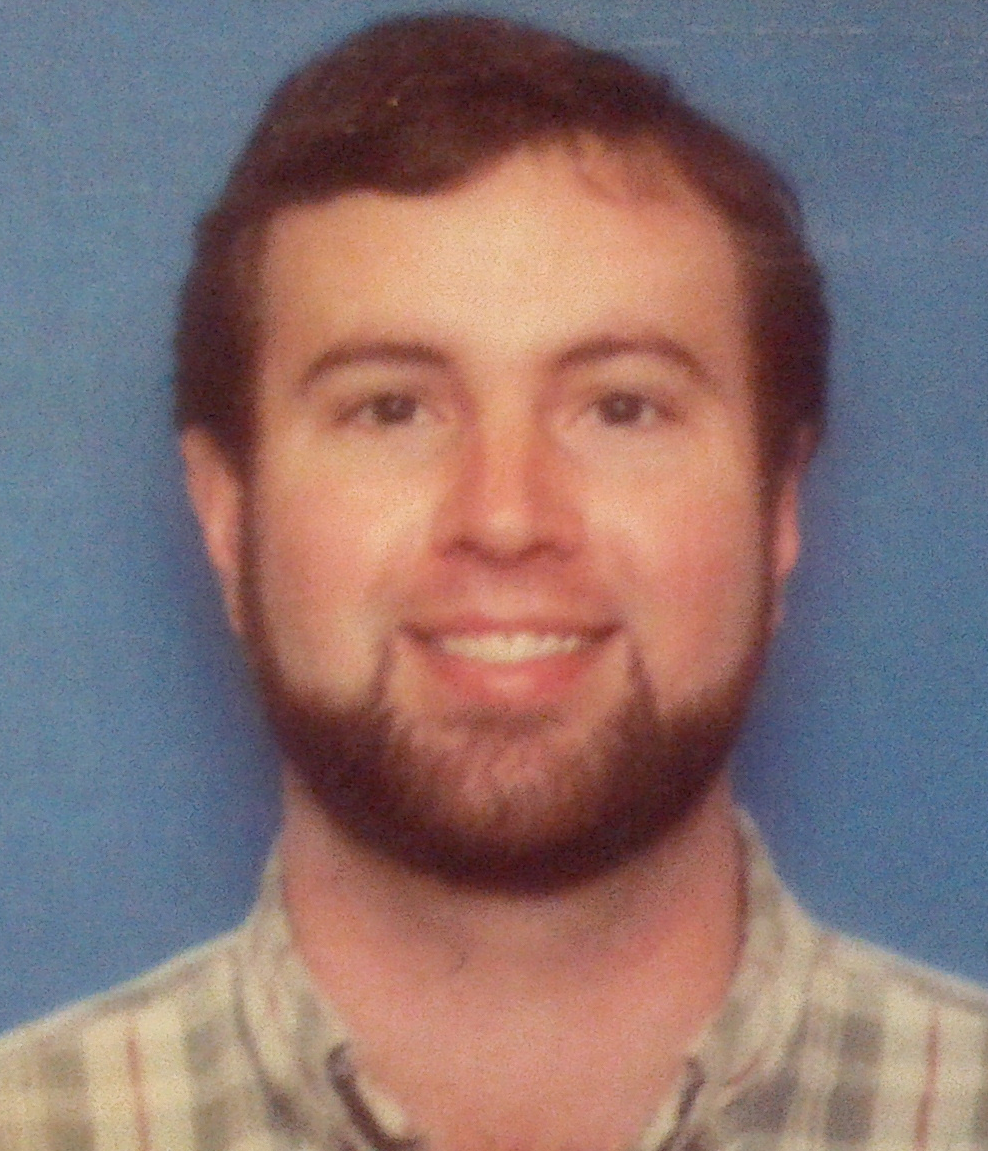
\includegraphics[width=1in,height=1.25in,clip,keepaspectratio]{main/data/dsmith.png}}]{Donnie Smith} 
(M'?)  has been a student of CS 6241 since Fall of 2012.  
\end{IEEEbiography}

\begin{IEEEbiography}[{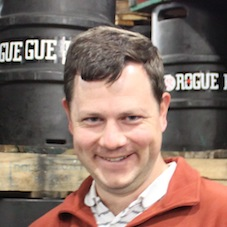
\includegraphics[width=1in,height=1.25in,clip,keepaspectratio]{main/data/kwharrigan.jpg}}]{Kyle Harrigan} 
(M'?) has been a student of CS 6241 since Fall of 2012.  
\end{IEEEbiography}

\end{document}  



